% Ubah judul dan label berikut sesuai dengan yang diinginkan.
\section{Arsitektur}
\label{sec:arsitektur}

% Ubah paragraf-paragraf pada bagian ini sesuai dengan yang diinginkan.
Pada penelitian ini dikembangkan suatu alat kontrol yang dapat menerima perintah melalui perangkat lain seperti laptop maupun Jetson Nano secara nirkabel. Pada sub bab ini akan dijabarkan implementasi dari alat yang dikembangkan pada penelitian ini.

Berikut ini dijabarkan beberapa \emph{Hardware} dan juga \emph{Software} yang digunakan pada penelitian ini seperti berikut:
\begin{enumerate}
    \item Anaconda Navigator
    \item Arduino IDE 
    \item Laptop 
    \item Jetson Nano
    \item Kamera
    \item ESP32 Devkit V1
    \item 2 Kontroller Motor
    \item 2 DC-DC Voltage Regulator
    \item 2 DC Motor
    \item Baterai 24V
\end{enumerate}

\subsection{Skematik Alat}
\label{subsec:skematik alat}

Skematik pada alat ini diilustrasikan secara rinci pada Gambar \ref{fig:Skematik Alat}. Sistem ini menggunakan kamera yang dihubungkan dengan Laptop atau Jetson Nano sebagai perangkat utama dalam menangkap citra. Proses kerja dimulai saat kamera menangkap citra objek. Citra yang telah ditangkap ini lantas diproses oleh Laptop atau Jetson Nano. Di dalam sistem ini, model klasifikasi yang telah diprogram sebelumnya memainkan peran penting dalam menginterpretasikan data citra tersebut. Hasil dari proses klasifikasi ini sangat krusial karena menjadi dasar dalam penentuan kode instruksi yang akan diimplementasikan.

Kode instruksi tersebut kemudian akan dikombinasikan dengan parameter kecepatam maksimal yang sebelumnya telah ditetapkan oleh pemngguna. Gabungan dari kode instruksi dan parameter kecepatan ini akan menjadi satu paket data sebagai kontrol gerak kursi roda. Paket data ini kemudian akan ditransmisikan secara nirkabel, baik dengan Bluetooth maupun WiFi, ke modul ESP32 Devkit V1. 

ESP32 memiliki peranan penting dalam kontrol motor kursi roda. ESP32 akan digunakan sebagai pusat pengendalian yang menerima paket data yang telah dikirimkan oleh pengguna secara nirkabel. Kemudian ESP32 akan melakukan pemecahan paket data dan menyesuaikan data tersebut kedalam variabel-variabel yang telah ditentukan. Proses pemecahan paket data ini akan menghasilkan dua data utama yang kemudian akan diproses lebih lanjut oleh ESP32.

Variabel pertama merupakan variabel arah yang memiliki fungsi krusial untuk menentukan arah gerak kedua motor pada kursi roda. Variabel ini akan memastikan bahwa motor bergerak sesuai dengan arah yang diinginkan sesuai dengan data yang diterima. Selain itu terdapat variabel kecepatan yang digunakan untuk menetapkan kecepatan maksimal pergerakan motor.

\begin{figure} [ht] \centering
  % Nama dari file gambar yang diinputkan
  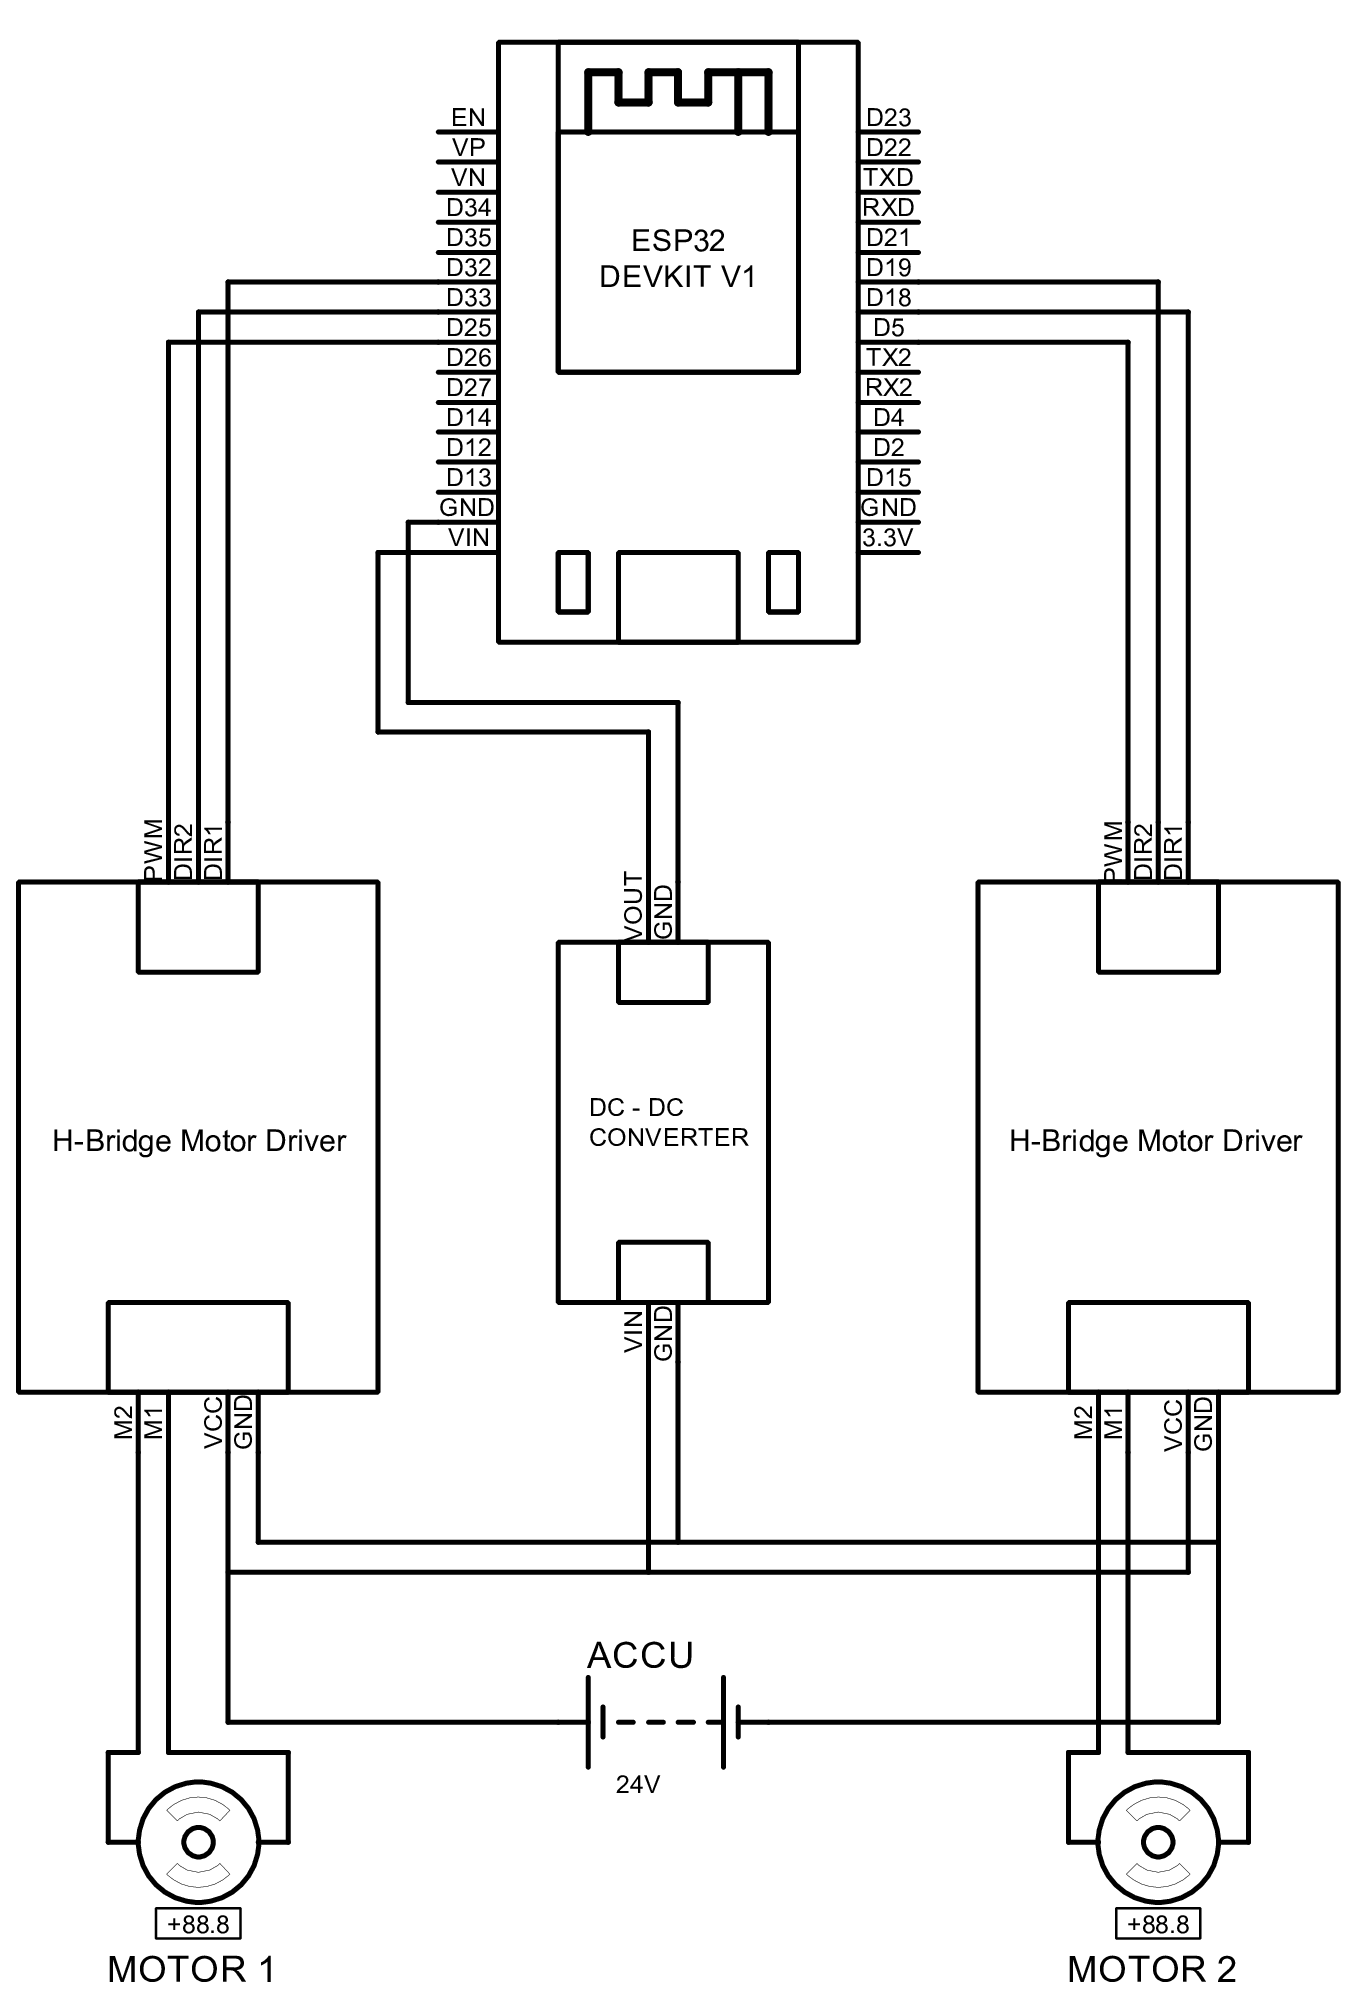
\includegraphics[scale=0.24]{gambar/bab3/Schematics.png}
  % Keterangan gambar yang diinputkan
  \caption{Skematik kontrol motor kursi roda}
  % Label referensi dari gambar yang diinputkan
  \label{fig:Skematik Alat}
\end{figure}

Dalam implementasinya terdapat serangkaian logika \emph{if} berantai yang akan dijelaskan secara terperinci pada sub bab program. Sederhananya logika \emph{if} berantai ini memiliki peran yang penting dalam pengambilan keputusan baik arah dan kecepatan motor sesuai dengan data yang telah diterima. Hasil dari logika ini akan memberikan \emph{trigger} berupa tegangan 5V ataupun 0V. Tegangan ini kemudian akan mempengaruhi arah putar motor.

Selanjutnya variabel kecepatan akan digunakan untuk mengatur tingkat \emph{Pulse Width Modulation} pada kontroler motor. Pengaturan PWM ini sangatlah penting guna mengatur kecepatan putar motor. Dengan mengatur tingkat PWM maka kecepatan motor maksimal dapat disesuaikan sesuai dengan kebutuhan.

